%%%%%%%%%%%%%%%%%%%%%%%%%
% !TEX TS-program = pdflatex
% !TEX root = ../tesis.tex
%%%%%%%%%%%%%%%%%%%%%%

%%%%%%%%%%%%%
%% DOCUMENT CLASS DEFINITIONS
%%%%%%%%%%%%%

\documentclass[b5paper,11pt]{book}
%\documentclass[a4paper,twoside,11pt,titlepage]{book}

%%%%%%%%%%%%%%%%%
%% INFORMACIÓN TESIS
%%%%%%%%%%%%%%%%%
\newcommand{\myTitle}{Thesis Title \xspace}
\newcommand{\mySubtitle}{Thesis\xspace}
\newcommand{\myDegree}{International PhD Degree in ...\xspace}
\newcommand{\myProgram}{Doctorate program \xspace}
\newcommand{\myName}{Author's name \xspace}
\newcommand{\myProf}{First Supervisor \xspace}
\newcommand{\myOtherProf}{Second Supervisor\xspace}
\newcommand{\myFaculty}{School of ... \xspace}
\newcommand{\myDepartment}{Department\xspace}
\newcommand{\myUni}{University of XXX \xspace}
\newcommand{\myLocation}{City \xspace}
\newcommand{\myTime}{Date of defense \xspace}


%%%%%%%%%%%%%
%% FONT
%%%%%%%%%%%%%
% https://tex.stackexchange.com/questions/426279/fontfamily-selectfont-does-not-work-with-xelatex-engine
% https://tug.org/FontCatalogue/sansseriffonts.html
% https://tug.org/FontCatalogue/

\usepackage[T1]{fontenc} 
\usepackage[utf8]{inputenc} 
\usepackage{libertine} 
\usepackage{libertinust1math} 

\usepackage[spanish,es-lcroman,english]{babel} 
\usepackage{microtype}


%%%%%%%%%%%%%%%%%%%
%% DESIGN SETTINGS
%%%%%%%%%%%%%%%%%%%
\usepackage{geometry}
  \geometry{
    paper=b5paper, % tamaño del papel
  	twoside, 
  	includehead, 
  	includefoot, 
  	right=20mm, left=20mm, 
  	bottom=10mm, 
  	bindingoffset=3mm,
  	top=10mm,   
  }


\geometry{hscale=0.75,vscale=0.8}

\geometry{textwidth=127.4818mm}


%%%%%%%%%%%%%
%% GRAPHICS
%%%%%%%%%%%%%
\usepackage{graphicx}    
\usepackage{subcaption} 
\usepackage{caption}
\captionsetup{
    font=small,
    labelfont={bf}
}

\usepackage{tikz}
\usetikzlibrary{decorations.pathreplacing}

%%%%%%%%%%%%%
%% TABLES
%%%%%%%%%%%%%    
\usepackage{booktabs} 

\usepackage{multirow} 

\usepackage{longtable} 

\usepackage{colortbl} 

\newcommand{\letratabla}{\fontsize{9}{11}\selectfont}

\usepackage{placeins}


%%%%%%%%%%%%%
%% MATH
%%%%%%%%%%%%

\usepackage{amssymb, amsmath, amsbsy}
\DeclareMathOperator{\sign}{sign} 


\usepackage[boxed]{algorithm2e} 
\newtheorem{theorem}{Theorem}[chapter]
\newtheorem{example}{Example}[chapter]
\newtheorem{definition}{Definition}[chapter]


\decimalpoint 

\usepackage{dcolumn}
\newcolumntype{.}{D{.}{\esperiod}{-1}}
\makeatletter
\addto\shorthandsspanish{\let\esperiod\es@period@code}
\makeatother




%%%%%%%%%%%%%%%
%% STYLE
%%%%%%%%%%%%%%%

%%% Definicion de COLORES
\definecolor{gray97}{gray}{.97}
\definecolor{gray85}{gray}{.85}
\definecolor{gray75}{gray}{.75}
\definecolor{gray45}{gray}{.45}
\definecolor{gray30}{gray}{.94}
\definecolor{plum_trad}{rgb}{0.56, 0.27, 0.52} 

\usepackage{indentfirst}

%%% Separate specific names
\hyphenation{A-na-to-mi-cal io-flu-pane lan-gua-ge Wi-lliams me-ta-bo-lic pipe-line}
\hyphenation{a-ccor-ding}
\hyphenation{ac-ti-vi-ty}
\hyphenation{ana-ly-ses}
\hyphenation{ana-ly-sis}
\hyphenation{cha-llen-ge}
\hyphenation{con-fi-gu-ra-tion}  
\hyphenation{co-rrec-ting}  
\hyphenation{du-mmi-es}  
\hyphenation{e-xa-mi-na-tion}  
\hyphenation{em-pi-ri-cal}  
\hyphenation{ins-ti-tu-tion} 
\hyphenation{i-ma-ge}
\hyphenation{neuro-i-ma-ging}
\hyphenation{i-ma-ging}
\hyphenation{ho-we-ver} 
\hyphenation{hy-po-the-sis} 
\hyphenation{fi-gu-re}  
\hyphenation{fo-llo-wed}   
\hyphenation{li-mi-ta-tion}
\hyphenation{ne-ver-the-less}  
\hyphenation{u-sing}  
\hyphenation{re-pre-sents}  
\hyphenation{pro-blems}  
\hyphenation{va-li-da-tion}  


\usepackage{enumitem}

%%% ENUMERACIÓN de SECCIONES
\setcounter{secnumdepth}{4} 
\setcounter{tocdepth}{3} 

\usepackage{minitoc}
\mtcsettitle{minitoc}{} 



%%%%%%%%%%%%%%%%%%%%%%%%
%% HEADER AND FOOT PAGE
%%%%%%%%%%%%%%%%%%%%%%%%
\usepackage{fancyhdr}

\usepackage[stable]{footmisc} 

\fancypagestyle{plain}{
  \fancyhf{} 
  \renewcommand{\headrulewidth}{0pt}
  \fancyfoot[CO,CE]{\textcolor{gray45}{\thepage}} % 
}


\pagestyle{fancy}
% O: odd E: even impar/par
% R: right L: left C: centre
\fancyhf{} 

\renewcommand{\chaptermark}[1]{\markboth{#1}{}} 
\renewcommand{\sectionmark}[1]{\markright{\thesection. #1}}


\fancyhead[LE]{\footnotesize\itshape\nouppercase{\leftmark}}
\fancyhead[RO]{\footnotesize\itshape\nouppercase{\rightmark}}
\setlength{\headheight}{14.5pt} 

\newcommand{\HRule}{\rule{\linewidth}{0.5mm}}


\fancyfoot[CO,CE]{\thepage}

\usepackage{etoolbox}
\makeatletter
\patchcmd{\f@nch@head}{\rlap}{\color{gray45}\rlap}{}{}
\patchcmd{\headrule}{\hrule}{\color{gray85}\hrule}{}{}
\patchcmd{\f@nch@foot}{\rlap}{\color{gray45}\rlap}{}{}
\makeatother

% BLANK PAGES
\makeatletter
\def\clearpage{%
  \ifvmode
    \ifnum \@dbltopnum =\m@ne
      \ifdim \pagetotal <\topskip
        \hbox{}
      \fi
    \fi
  \fi
  \newpage
  \thispagestyle{empty}
  \write\m@ne{}
  \vbox{}
  \penalty -\@Mi
}
\makeatother

%%%%%%%%%%%%%
%%  TITLES
%%%%%%%%%%%%%

\usepackage{titlesec}
  
\newcommand{\hsp}{\hspace{15pt}}    
\titleformat{\chapter}[hang]
{\Huge\bfseries}{\textcolor{gray45}{\thechapter}\hsp\textcolor{gray45}{|}\hsp}{0pt}{\LARGE\bfseries\MakeUppercase}

\titleformat{\part}[display]
{\centering\huge\bfseries}
{Part \thepart}
{1em}
{\Huge\bfseries\MakeUppercase}

\assignpagestyle{\part}{empty}


%%%%%%%%%%%%%%%%%%%%%%%%%%%%%%%%
%% INDEX
%%%%%%%%%%%%%%%%%%%%%%%%%%%%%%%%


\usepackage{tocloft} 

\setlength{\cftfigindent}{0pt} 
\renewcommand{\cftfigpresnum}{Figure } 
\addtolength{\cftfignumwidth}{3.5em} 

\setlength{\cfttabindent}{0pt} 
\renewcommand{\cfttabpresnum}{Table } 
\addtolength{\cfttabnumwidth}{2.5em} 


%%%%%%%%%%%%%
%%  REFERENCES
%%%%%%%%%%%%
\usepackage{url} 

\usepackage[bookmarks = true, colorlinks=true, linkcolor = black, citecolor = black, menucolor = black, urlcolor = black]{hyperref} 

\hypersetup{
pdfauthor = {\myName email},
pdftitle = {\myTitle},
pdfsubject = {},
pdfkeywords = {aaaa, bbbb},
pdfcreator = {LaTeX},
pdfproducer = {pdflatex}
}


%%%%%%%%%%%%%
%% CODE
%%%%%%%%%%%%%
\usepackage{listings} 

\lstset{ frame=Ltb,                 
     framerule=0.5pt,              
     aboveskip=0.5cm,             
     framextopmargin=3pt,     
     framexbottommargin=3pt, 
     framexleftmargin=0.1cm, 
     framesep=0pt, 
     rulesep=.4pt, 
     backgroundcolor=\color{gray97}, 
     rulesepcolor=\color{black}, 
     stringstyle=\ttfamily, 
     showstringspaces = false, 
     basicstyle=\scriptsize\ttfamily, 
     commentstyle=\color{gray45}, 
     keywordstyle=\bfseries, 
     %
     numbers=left, 
     numbersep=6pt,
     numberstyle=\tiny,
     numberfirstline = false,
     breaklines=true, 
   }
 
\lstnewenvironment{listing}[1][] 
   {\lstset{#1}\pagebreak[0]}{\pagebreak[0]} 


\lstdefinestyle{CodigoC}
   {
	basicstyle=\scriptsize,
	frame=single,
	language=C,
	numbers=left
   }
\lstdefinestyle{CodigoC++}
   {
	basicstyle=\small,
	frame=single,
	backgroundcolor=\color{gray30},
	language=C++,
	numbers=left
   }

 
\lstdefinestyle{Consola}
   {basicstyle=\scriptsize\bf\ttfamily,
    backgroundcolor=\color{gray30},
    frame=single,
    numbers=none
   }


\newcommand{\bigrule}{\titlerule[0.5mm]}


%%%%%%%%%%%%%
%%  GLOSSARY
%%%%%%%%%%%%

\usepackage[smaller,printonlyused]{acronym} 



%%%%%%%%%%%%%
%%  BIBLIOGRAPHY
%%%%%%%%%%%%
\usepackage{bibentry} 
\nobibliography*

\usepackage{breakcites} 



%[htbp]: here (h), top (t), bottom (b), top of next page (p). With [H], you tell LaTeX to put the image exactly there. To use [H] you have to load the {float} package.

% To search for faults in a character, if you don't know what it is, you can apply the following:
%\DeclareUnicodeCharacter{0301}{*************************************}


\begin{document}
\dominitoc

\pagenumbering{roman}

%%%%%% Si estuviera en español
%\renewcommand{\listtablename}{Índice de tablas} 
%\renewcommand{\tablename}{Tabla}

%%%%%%%%%%%%%%%%%
%% FRONT COVER AND SIMILAR
%%%%%%%%%%%%%%%%%
\frontmatter
\begingroup
% !TEX TS-program = pdflatex
% !TEX root = ../tesis.tex
%%%%%%%%%%%%%%%%%%%%%%
%% PORTADA
%%%%%%%%%%%%%%%%%%%%%%


\begin{titlepage}
\pdfbookmark{Titlepage}{Titlepage}

\newlength{\centeroffset}
\setlength{\centeroffset}{-0.5\oddsidemargin}
\addtolength{\centeroffset}{0.5\evensidemargin}

\thispagestyle{empty}

\noindent\hspace*{\centeroffset}\begin{minipage}{\textwidth}

%\centering
%
\includegraphics[width=0.7\textwidth]{Figures/logo_ugr}\\[1cm]


\centering

\includegraphics[width=0.35\textwidth]{Figures/logo_ugr2}\\[0.5cm]

{\large PhD Thesis \\}
%{ \myProgram }
%\vspace{0.5cm}
%{\large \myProgram \\}

\vspace{1cm}

\rule{\linewidth}{0.1mm}
\vspace{0.06cm}

{\Large \MakeUppercase{ \textbf{\myTitle}} \\ }

\vspace{0.3cm}		
\rule{\linewidth}{0.1mm}	

%\noindent\rule[-1ex]{\textwidth}{3pt}\\[3.5ex]
%{\large\bfseries Subtítulo del proyecto.\\[4cm]}
\end{minipage}

\vspace{2cm}
\noindent\hspace*{\centeroffset}\begin{minipage}{\textwidth}
\centering

{\Large \textbf{Author:}\\[0.3cm]
{\Large  \myName}}\\[1.4cm]


{\large \textbf{Supervisors:}}\\[0.3cm]
{\large \myProf\\
\myOtherProf\\ [1cm]}

\vspace{0.3cm}
{\normalsize  \myProgram } \\ [0.7cm]
%\vspace{0.3cm}
%{ \myDepartment } \\[1cm]


%\includegraphics[width=0.15\textwidth]{imagenes/tstc.png}\\[0.1cm]
%\textbf{Departamento}\\
%{Electrónica y Tecnología de los Computadores}\\
%\textsc{---}\\
%{\small \myLocation, \myTime}
{\small \myTime}


		
\end{minipage}
%\addtolength{\textwidth}{\centeroffset}
%\vspace{\stretch{2}}

\end{titlepage}




\cleardoublepage

\thispagestyle{empty}

\noindent\hspace*{\centeroffset}\begin{minipage}{\textwidth}

\centering

\vspace{3.5cm}

{\LARGE \textbf{\myTitle} \\ } 
\vspace{1cm}
\begin{tikzpicture}[scale=0.05]
\draw[thick, domain=0:720, samples=100] plot (\x:{\x/100});
\end{tikzpicture}

\end{minipage}

\vspace{1cm}
\noindent\hspace*{\centeroffset}\begin{minipage}{\textwidth}
\centering

{\Large  \myName}\\ [0.2cm]
{\fontfamily{qcr}\selectfont
\href{mailto:aaaaa@edu.com}{aaaaa@edu.com}
} \\ [2.5cm]


\textbf{THESIS SUPERVISORS}\\[0.3cm]
{Dr. \myProf\\ [0.1cm]
{\small \textit{Research group (University of XXX)}} \\[0.3cm]
Dr. \myOtherProf\\ [0.1cm]
{\small \textit{Research group (University of XXX)}} \\ 
}
		
\end{minipage}


\clearpage
% !TEX TS-program = pdflatex
% !TEX root = ../tesis.tex

%*******************************************************
% Titleback
%*******************************************************
\thispagestyle{empty}



\begin{center}
{\large PhD Thesis} \\[0.15cm] 
{\large  \myProgram}
\end{center}


\hfill

\vspace{\stretch{1}}


\medskip


\noindent
{\large \textbf{Funding}}\\ [0.2cm]
Include here funding information \\[1.5cm]







\cleardoublepage
%*******************************************************
% Dedication
%*******************************************************
%\cleardoubleemptypage
\thispagestyle{empty}
%\phantomsection 
%\refstepcounter{dummy}
%\pdfbookmark[1]{Dedication}{Dedication}

\vspace*{3cm}

\begin{flushright}
{\small	\textit{You must always have faith in people. And most importantly, \\you must always have faith in yourself.} \\ \medskip
	--- Elle Woods (Legally Blonde, 2001)}
\end{flushright}




% !TEX TS-program = pdflatex
% !TEX root = ../Tesis.tex

%*******************************************************
% Acknowledgements
%*******************************************************
\pdfbookmark{Acknowledgements}{Acknowledgements}


\chapter*{ACKNOWLEDGEMENTS}

Lorem ipsum dolor sit amet, consectetur adipiscing elit. Sed do eiusmod tempor incididunt ut labore et dolore magna aliqua. Ut enim ad minim veniam, quis nostrud exercitation ullamco laboris nisi ut aliquip ex ea commodo consequat.




\cleardoublepage

%%%%%%%%%%%%%%%%%%%%%%%%%
% !TEX TS-program = pdflatex
% !TEX root = ../tesis.tex
%%%%%%%%%%%%%%%%%%%%%%

%*******************************************************
% Abstract
%*******************************************************
%\renewcommand{\abstractname}{Abstract}
\pdfbookmark[0]{Abstract}{Abstract}

%\let\clearpage\relax
%\let\cleardoublepage\relax
%\let\cleardoublepage\relax

\chapter*{ABSTRACT}

This is filler text. This is filler text. This is filler text. This is filler text. This is filler text. This is filler text. This is filler text. This is filler text. This is filler text.


\vfill
\cleardoublepage
%%%%%%%%%%%%%%%%%%%%%%%%%
% !TEX TS-program = pdflatex
% !TEX root = ../tesis.tex
%%%%%%%%%%%%%%%%%%%%%%


%*******************************************************
% Abstract
%*******************************************************
%\renewcommand{\abstractname}{Abstract}

%\let\clearpage\relax
%\let\cleardoublepage\relax
%\let\cleardoublepage\relax
%\thispagestyle{plain}

\begin{otherlanguage}{spanish}
\pdfbookmark[0]{Resumen}{Resumen}
\chapter*{RESUMEN AMPLIO EN CASTELLANO}

\section*{Motivación}
Lorem ipsum dolor sit amet, consectetur adipiscing elit. Sed do eiusmod tempor incididunt ut labore et dolore magna aliqua. Ut enim ad minim veniam, quis nostrud exercitation ullamco laboris nisi ut aliquip ex ea commodo consequat.


\section*{Objetivos}

Lorem ipsum dolor sit amet, consectetur adipiscing elit. Sed do eiusmod tempor incididunt ut labore et dolore magna aliqua. Ut enim ad minim veniam, quis nostrud exercitation ullamco laboris nisi ut aliquip ex ea commodo consequat.


\section*{Contribuciones}
Lorem ipsum dolor sit amet, consectetur adipiscing elit. Sed do eiusmod tempor incididunt ut labore et dolore magna aliqua. Ut enim ad minim veniam, quis nostrud exercitation ullamco laboris nisi ut aliquip ex ea commodo consequat.


\section*{Conclusiones}
Lorem ipsum dolor sit amet, consectetur adipiscing elit. Sed do eiusmod tempor incididunt ut labore et dolore magna aliqua. Ut enim ad minim veniam, quis nostrud exercitation ullamco laboris nisi ut aliquip ex ea commodo consequat.


\end{otherlanguage}

		


\cleardoublepage

%%%%%%%%%%%%%%%%%
%% INDEX
%%%%%%%%%%%%%%%%%

%\pagestyle{plain}
\pdfbookmark[0]{\contentsname}{tableofcontents}
%\renewcommand{\contentsname}{CONTENTS}
\tableofcontents
\cleardoublepage
\pdfbookmark[0]{\listfigurename}{lof}
%\renewcommand{\listfigurename}{LIST OF FIGURES}
\listoffigures 
\cleardoublepage
\pdfbookmark[0]{\listtablename}{lot}
%\renewcommand{\listtablename}{ LIST OF TABLES}
\listoftables
\cleardoublepage
\pdfbookmark[0]{Acronyms}{acronyms}
\chapter*{ACRONYMS}
\markboth{Acronyms}{Acronyms}
% When any of these words are mentioned in the text, you have to write \ac and its reduced version
% first ac{cd}\ % The first time the full name and abbreviation
% second ac{cd}\ % The rest of the times the abbreviation 
% long & acl{cd} % if you want full name
% short  acs{cd} % if you want only abbreviation
% full  acf{} % if you want full name and abbreviation
% plural \acp{} % plural


\begin{acronym}[LIME] % To define the space, the longest abbreviation is used.
    \acro{AD}{Alzheimer's Disease}
    \acro{CNN}{Convolutional Neural Network}
    \acro{LIME}{Local Interpretable Model-agnostic Explanations}
    \acro{SPM}{Statistical Parametric Mapping}
    \acro{XAI}{Explainable Artificial Intelligence}

    
 \end{acronym}
\cleardoublepage
%{\listoftables \let\cleardoublepage\clearpage \printglossary[type=\acronymtype, title=Acrónimos ]}
%\printglossary[type=\acronymtype, title=ACRONYMS]
\endgroup

%%%%%%%%%%%%%%%%%
%% CONTENT
%%%%%%%%%%%%%%%%%
\mainmatter
\pagenumbering{arabic}
\setlength{\parskip}{5pt}

\part{Fundamentals}\label{part1}
%%%%%%%%%%%%%%%%%%%%%%%%%
% !TEX TS-program = pdflatex
% !TEX root = ../tesis.tex
%%%%%%%%%%%%%%%%%%%%%%
%% CHAPTER 1
%%%%%%%%%%%%%%%%%%%%%%

\chapter{Introduction}\label{chap_01}
%%%%%%%%%%%%%%%%%%%%%%%%%
\minitoc
%\clearpage

\section{Motivation}\label{sec_motivation}

This template has been created specifically for the defence of Thesis~\cite{tesis}. If you make use of this template or base your work on it, please provide proper attribution or reference to its original source.



\section{Aims and objectives}\label{sec_aims}

This template uses the \texttt{acronym} package to manage abbreviations consistently throughout the text. Acronyms should be defined inside the \texttt{acronym} environment and referenced in the text using dedicated commands. The usage is summarised below:

\begin{itemize}
    \item \verb|\ac{cd}| — On first use, prints the full name followed by the acronym in parentheses: \ac{CNN}. Later uses show only the acronym: \ac{CNN}.
    
    \item \verb|\acs{cd}| — Prints only the short form (the acronym), even on first use: \acs{AD}.
    
    \item \verb|\acl{cd}| — Prints only the long form (the full name): \acl{CNN}.
    
    \item \verb|\acf{cd}| — Always prints the full name and acronym: \acf{AD}.
    
    \item \verb|\acp{cd}| — Prints the plural form, automatically adding an “s” to the acronym and adjusting the long form if defined: \acp{CNN}.
\end{itemize}

All acronyms must be defined in the \texttt{acronym} environment.


\section{Organisation of this thesis}\label{sec_organization}

This thesis is organised... It is divided into various topics and chapters as illustrated in Figure~\ref{fig:01_objetivos}.

\begin{figure*}[htbp]
\centering
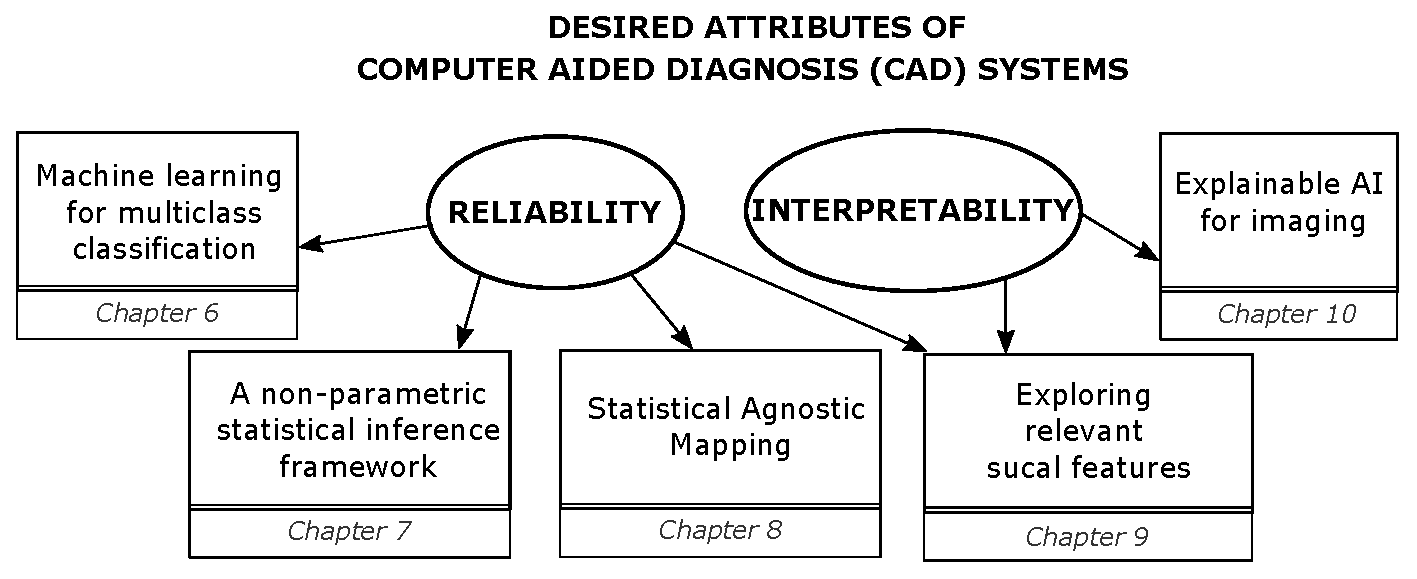
\includegraphics[width=0.8\textwidth]{Figures/chap_01/objetivos}
\caption{Structured scheme of the content of the contributions of this thesis. }
\label{fig:01_objetivos}
\end{figure*}


\section{Contributions}\label{sec_controbutions}

Part of the content of this thesis, including figures and tables, has been published in several international journal articles and conference presentations. These contributions are detailed below.

\subsection*{Articles}

\bibentry{JimenezMesa2020} (\textbf{chapter~\ref{chap_04}})


\subsection*{Conferences}

\bibentry{JimenezMesa2020} (\textbf{chapter~\ref{chap_04}})




 % Introduction
%%%%%%%%%%%%%%%%%%%%%%%%%
% !TEX TS-program = pdflatex
% !TEX root = ../tesis.tex
%%%%%%%%%%%%%%%%%%%%%%
%% CHAPTER 2
%%%%%%%%%%%%%%%%%%%%%%

%%%%%%%%%%%%%%%%%%%%%%%%%
\chapter{Fundamentals}\label{chap_02}
%%%%%%%%%%%%%%%%%%%%%%%%%
\minitoc

\vspace{1cm}


In this chapter...

\section{New section}
This is filler text. This is filler text. This is filler text. This is filler text. This is filler text. This is filler text. This is filler text. This is filler text. This is filler text.

This is filler text. This is filler text. This is filler text. This is filler text. This is filler text. This is filler text. This is filler text. This is filler text. This is filler text.






 % Fundamentals
%\input{Chapters/chap_03}
%\input{Chapters/chap_03_2}
%\input{Chapters/chap_03_3}

\part{Contributions of this thesis}\label{part2}
%%%%%%%%%%%%%%%%%%%%%%%%%
% !TEX TS-program = pdflatex
% !TEX root = ../tesis.tex
%%%%%%%%%%%%%%%%%%%%%%
%% CHAPTER 4
%%%%%%%%%%%%%%%%%%%%%%

%%%%%%%%%%%%%%%%%%%%%%%%%
\chapter{Application of ...}\label{chap_04}
%%%%%%%%%%%%%%%%%%%%%%%%%
\minitoc
% Define the algorithm per chapter (it has to be put in each chapter where one is put in).
\setcounter{algocf}{0} % Reset the algorithm counter in each chapter
\renewcommand{\thealgocf}{\thechapter.\arabic{algocf}} % Numbering of algorithms by chapters

\vspace{1cm}


\section{Introduction}

Lorem ipsum dolor sit amet, consectetur adipiscing elit. Sed do eiusmod tempor incididunt ut labore et dolore magna aliqua. Ut enim ad minim veniam, quis nostrud exercitation ullamco laboris nisi ut aliquip ex ea commodo consequat.



\section{Methodology}

Lorem ipsum dolor sit amet, consectetur adipiscing elit. Sed do eiusmod tempor incididunt ut labore et dolore magna aliqua. Ut enim ad minim veniam, quis nostrud exercitation ullamco laboris nisi ut aliquip ex ea commodo consequat.


\section{Results}

This is a placeholder paragraph intended to demonstrate the layout and formatting of the text. The actual content will be written here once the structure of the thesis is defined and the main arguments are developed accordingly.

Figure~\ref{fig:regions} illustrates...

\begin{figure}[!h]
  \centering
 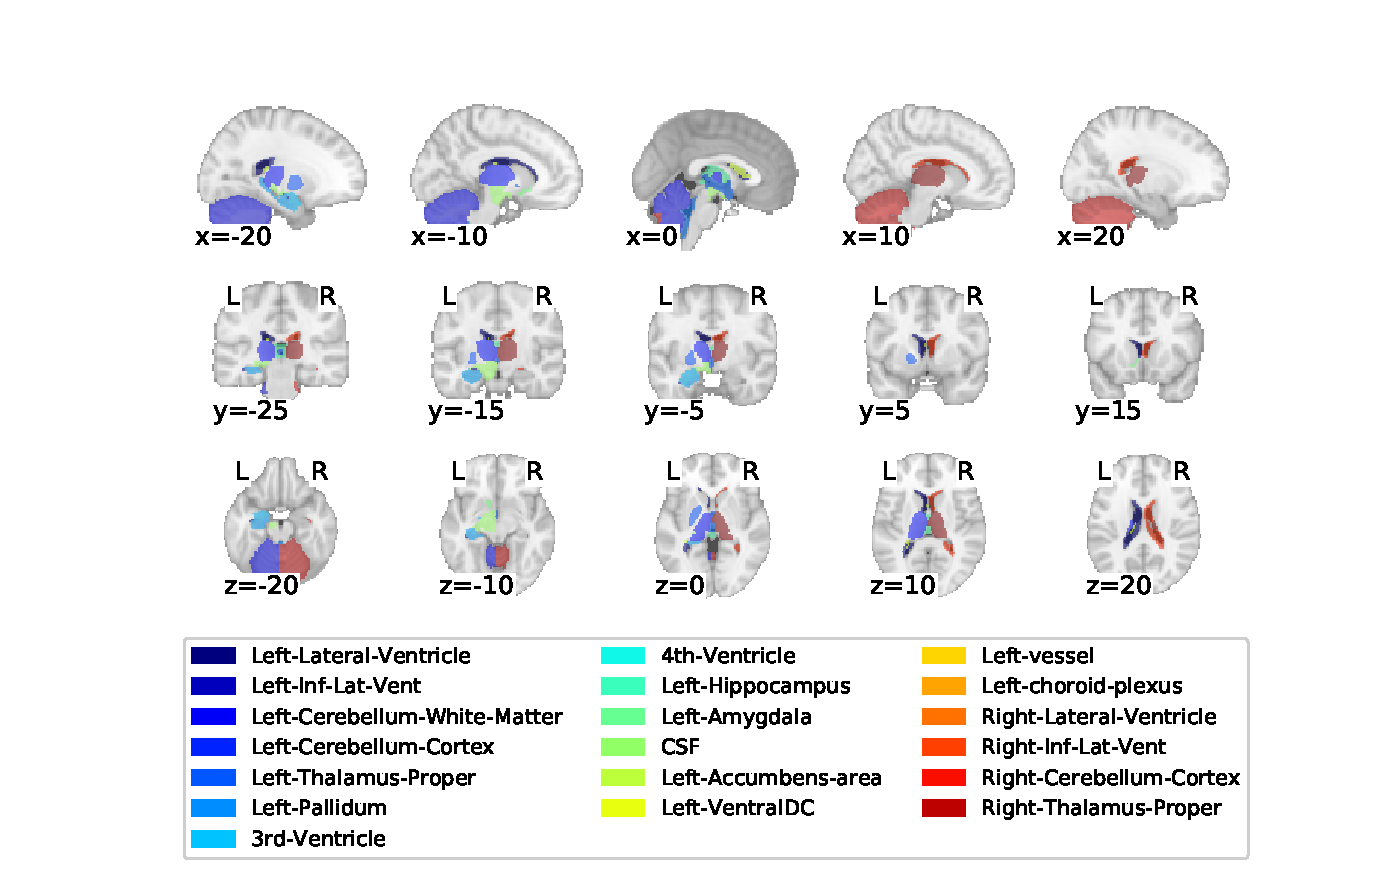
\includegraphics[width=0.7\textwidth]{Figures/chap_04/ROI7}
\caption{Selected regions after one-vs-one $t$-test feature selection.}\label{fig:regions}
\end{figure}

Table~\ref{tab:all} summarises ...

\begin{table}[htb]
\centering
\resizebox{0.8\textwidth}{!}{ \begin{tabular}{ccccccccc}
\toprule
\multicolumn{2}{l}{ }    & \multicolumn{3}{l}{\textbf{Training}}   &     & \multicolumn{3}{l}{ \textbf{Test (without dummies)}}  \\
\textbf{Ensemble} & \textbf{Classifier}  & Accuracy & Recall &F1-score & & Accuracy & Recall &F1-score \\
\midrule
-& SVM lineal              & 0.48     & 0.47   & 0.47   & & \textbf{0.67}   & \textbf{0.52}     & \textbf{0.66} \\
-& SVM RBF                 & 0.47     & 0.47   & 0.48   & &  0.67   & 0.52  & 0.63 \\
LogitBoost& Decision Tree & 0.48  & 0.44   & 0.51   &  & 0.64   & 0.46     & 0.60 \\
Random forest&Decision Tree & 0.48     & 0.44   & 0.52 & & 0.64   & 0.51     & 0.57 \\
AdaBoost&Decision Tree   & 0.50     & 0.42   & 0.47  &  & 0.60   & 0.43     & 0.52 \\
-&                  $5$-NN & 0.52     & 0.43   & 0.44  &  & 0.60   & 0.44     & 0.46 \\
-&                   $1$-NN & 0.52     & 0.39  & 0.42  & &  0.58   & 0.39     & 0.44 \\
-&                  $3$-NN & 0.51     & 0.40   & 0.39  & &  0.58   & 0.41     & 0.40 \\
-&                   MLP & 0.56     & 0.57   & 0.56  & &  0.60   & 0.60    & 0.59 \\
-&                   \acs{CNN} & 0.55     & 0.55  & 0.54  & &  0.48   & 0.47     & 0.48 \\
\bottomrule
 \multicolumn{6}{@{}l}{{\letratabla NN stands for nearest neighbours.}}
\end{tabular}}
\caption{Performance results for selected features using different classifiers.}\label{tab:all}
\end{table}


\section{Discussion}

Lorem ipsum dolor sit amet, consectetur adipiscing elit. Sed do eiusmod tempor incididunt ut labore et dolore magna aliqua. Ut enim ad minim veniam, quis nostrud exercitation ullamco laboris nisi ut aliquip ex ea commodo consequat.
 
%\input{Chapters/chap_05} 
%\input{Chapters/chap_06} 

\part{General discussion and conclusions}\label{part3}
%%%%%%%%%%%%%%%%%%%%%%%%%
% !TEX TS-program = pdflatex
% !TEX root = ../tesis.tex
%%%%%%%%%%%%%%%%%%%%%%
%% DISCUSSION AND CONCLUSIONS
%%%%%%%%%%%%%%%%%%%%%%


%%%%%%%%%%%%%%%%%%%%%%%%%
\chapter[General Discussion and Conclusions]{General Discussion and\\ Conclusions}\label{chap_09}
%%%%%%%%%%%%%%%%%%%%%%%%%
\minitoc

\section{General Discussion}

The contributions presented in this thesis have already been extensively discussed in their respective chapters within Part~\ref{part2}. In this final chapter, the focus will be on evaluating the impact of this work on ...

\subsection{Discussion on...}

\section{Conclusions and Future work}
%Introduction
Lorem ipsum dolor sit amet, consectetur adipiscing elit. Sed do eiusmod tempor incididunt ut labore et dolore magna aliqua. Ut enim ad minim veniam, quis nostrud exercitation ullamco laboris nisi ut aliquip ex ea commodo consequat.


%%%%%%%%%%%%%%%%%%%%%%%%%%%%%%%%%%%%%%%%%%%%%
%%%%%%%%%%%%%%%%%%%%%%%%%%%%%%%%%%%%%%%%%%%%%
%%%%%%%%%%%%%%%%%%%%%%%%%%%%%%%%%%%%%%%%%%%%%
% Conclusions

Lorem ipsum dolor sit amet, consectetur adipiscing elit. Sed do eiusmod tempor incididunt ut labore et dolore magna aliqua. Ut enim ad minim veniam, quis nostrud exercitation ullamco laboris nisi ut aliquip ex ea commodo consequat.


%%%%%%%%%%%%%%%%%%%%%%%%%%%%%%%%%%%%%%%%%%%%%
%%%%%%%%%%%%%%%%%%%%%%%%%%%%%%%%%%%%%%%%%%%%%
%%%%%%%%%%%%%%%%%%%%%%%%%%%%%%%%%%%%%%%%%%%%%
%% Future work

Lorem ipsum dolor sit amet, consectetur adipiscing elit. Sed do eiusmod tempor incididunt ut labore et dolore magna aliqua. Ut enim ad minim veniam, quis nostrud exercitation ullamco laboris nisi ut aliquip ex ea commodo consequat.



%\input{Chapters/chap_10}

%%%%%%%%%%%%%%%%%
%% APENDIX
%%%%%%%%%%%%%%%%%
\appendix
\part{Appendix}
%%%%%%%%%%%%%%%%%%%%%%%%%
% !TEX TS-program = pdflatex
% !TEX root = ../tesis.tex
%%%%%%%%%%%%%%%%%%%%%%
%% APENDICE 1
%%%%%%%%%%%%%%%%%%%%%%

%%%%%%%%%%%%%%%%%%%%%%%%%
\chapter[Supplementary Material for ...]{supplementary Material for ... \\ ...}\label{Apend:chap_04}
%%%%%%%%%%%%%%%%%%%%%%%%%
\minitoc

\vspace{1cm}

This chapter includes supplementary material related to chapter~\ref{chap_04}. Such material includes...

\section{Appendix}\label{appe:01}
Lorem ipsum dolor sit amet, consectetur adipiscing elit. Sed do eiusmod tempor incididunt ut labore et dolore magna aliqua. Ut enim ad minim veniam, quis nostrud exercitation ullamco laboris nisi ut aliquip ex ea commodo consequat.




%%%%%%%%%%%%%%%%%
%% BIBLIOGRAPHY
%%%%%%%%%%%%%%%%%


%\nocite{*}
\bibliographystyle{ieeetr}
\bibliography {Biblio/refs_tesis}
\addcontentsline{toc}{part}{Bibliography}



\end{document}
